\section{\uppercase{Experimental evaluation}}\label{sec:results}

\noindent Several tests were conducted in the simulated environments presented earlier for evaluating the ability of the proposed system to find suitable constellations of sensors for maximizing the observable surface area of a given set of target objects.

In the active perception environment introduced in \cref{fig:active-perception-environment}, it was performed two tests with the sensor deployment shown in \cref{fig:sensors-deployment-active-perception-environment}. In the first test it was estimated the best sensor position for observing a single target object (green starter motor) being occluded by a human hand starting to grasp it. By visually inspecting the scene in \cref{fig:active-perception-1-sensor}, it can be seen that the system chose a very reasonable sensor position, achieving a surface coverage of 27.73\%, despite the heavy occlusions present. Moreover, when expanding the number of sensors to 3 (in the second test), the system managed to select a sensor constellation with a good spatial distribution (shown in \cref{fig:active-perception-3-sensors}) that managed to improve the sensor coverage to 61.91\%.

Moving to the single bin picking environments, presented in \cref{fig:bin-picking-environment,fig:bin-picking-with-occlusions-environment}, it was made four more tests using the deployed sensors seen in \cref{fig:sensors-deployment-bin-picking-environments}. In the first test it was estimated the best position for a single sensor to observe the target object that was inside the stacking box, which had large occlusions on its surroundings, but could be clearly observed from above. As can be seen in \cref{fig:bin-picking-1-sensor}, the system choose a suitable observation sensor that managed to achieve a surface coverage of 45.10\%. When increasing the number of sensors to 5 (in the second test), the system relied on more sensor data and improved the surface coverage to 64.63\%. To make the active perception for this bin picking use case more challenging, it was added three occluding differential gearboxes on top of the target object (scene shown on \cref{fig:bin-picking-with-occlusions-environment}) in order to create large occlusions that significantly reduced the number of useful sensors in the deployed populations (presented in \cref{fig:sensors-deployment-bin-picking-environments}). Analyzing the best sensor position estimated by the system (shown in \cref{fig:sensor-data-processing,fig:bin-picking-with-occlusions-1-sensor}) it can be seen that the pose chosen was very reasonable, achieving a surface coverage of 19.27\%. When increasing the number of sensors to 3, the system deployed a constellation with good spatial distribution and managed to improved the surface coverage percentage of the target object to 31.19\% (as can be seen in \cref{fig:bin-picking-with-occlusions-3-sensors}).

Increasing the level of complexity even further, in the final test it was added three more target objects to the simulation environment (as presented in \cref{fig:multiple-bin-picking-with-occlusions-environment}) and the number of populations with different sensor types was increased to 7 (shown in \cref{fig:sensors-deployment-multiple-bin-picking-environment}). Analyzing \cref{fig:multiple-bin-picking-with-occlusions-10-sensors} in which the system estimated a constellation of 10 sensors to observe the 4 target objects, it can be seen that the system chose 4 sensors on the front wall (which had a better observation area for the target objects in the trolley shelves), 3 on the ceiling (for retrieving sensor data for the target objects on top of the trolley) and then for observing the remaining surface areas of the target objects, it chose one sensor on the left wall, another on the right wall and finally another one on the back wall, reaching 10 sensors in total and achieving a surface coverage of the target objects of 43.93\%.

These 7 constellations of sensors computed using \cref{alg:best-n-views} (which relied on a \gls{ransac} approach), show that the proposed system can estimate a suitable sensor configuration for maximizing the observable surface area of several target objects even on complex environments with significant occlusions. Moreover, the system managed to compute useful solutions in bounded and reasonable time (from less than a second to a few minutes depending on the number and characteristics of the deployed sensors) for a problem that is combinatorial explosive in terms of processing time complexity.

\begin{figure}
	\centering
	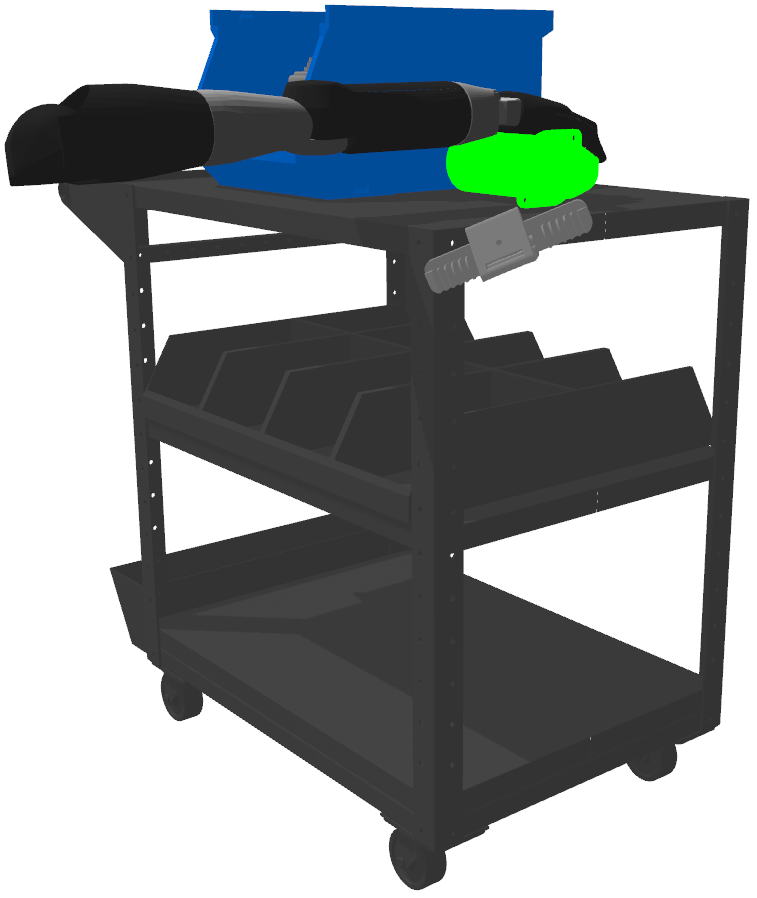
\includegraphics[height=.2\textwidth]{best-views-estimation/active-perception/1-sensor/gazebo-corner}\hspace{4em}
	\includegraphics[height=.2\textwidth]{best-views-estimation/active-perception/1-sensor/rviz-front-corner}\\
	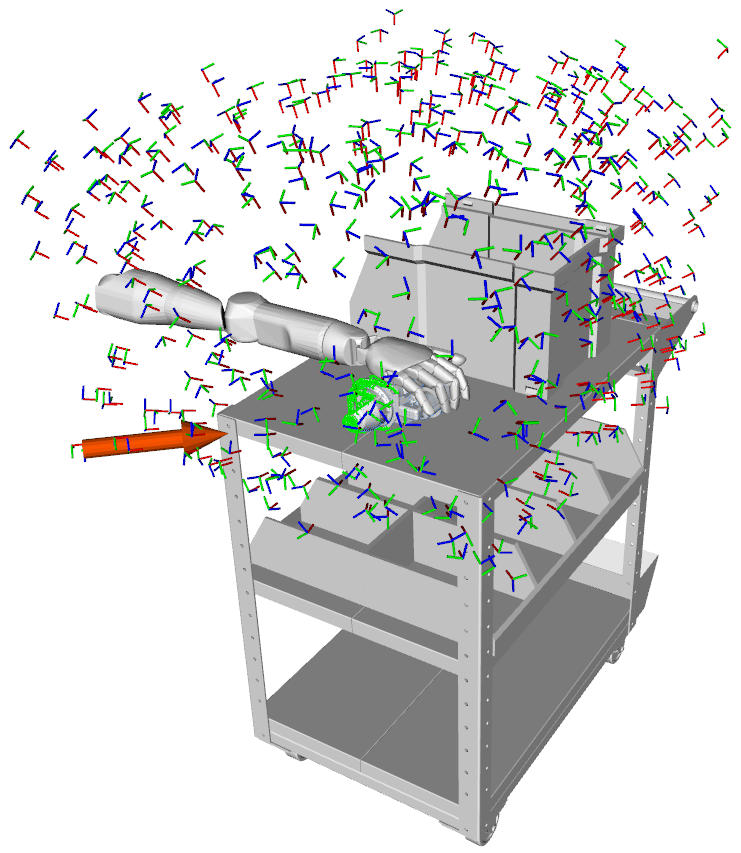
\includegraphics[height=.2\textwidth]{best-views-estimation/active-perception/1-sensor/rviz-back-corner}\hspace{2em}
	\includegraphics[height=.2\textwidth]{best-views-estimation/active-perception/1-sensor/rviz-top}
	\caption{Estimation of the best sensor position for the active perception environment with a 27.73\% of surface area coverage (top left showing the Gazebo color rendering and remaining images displaying the best sensor as a large red arrow, the deployed sensors as small coordinate frames and the observed sensor data as green spheres).}
	\label{fig:active-perception-1-sensor}
\end{figure}

\begin{figure}
	\centering
	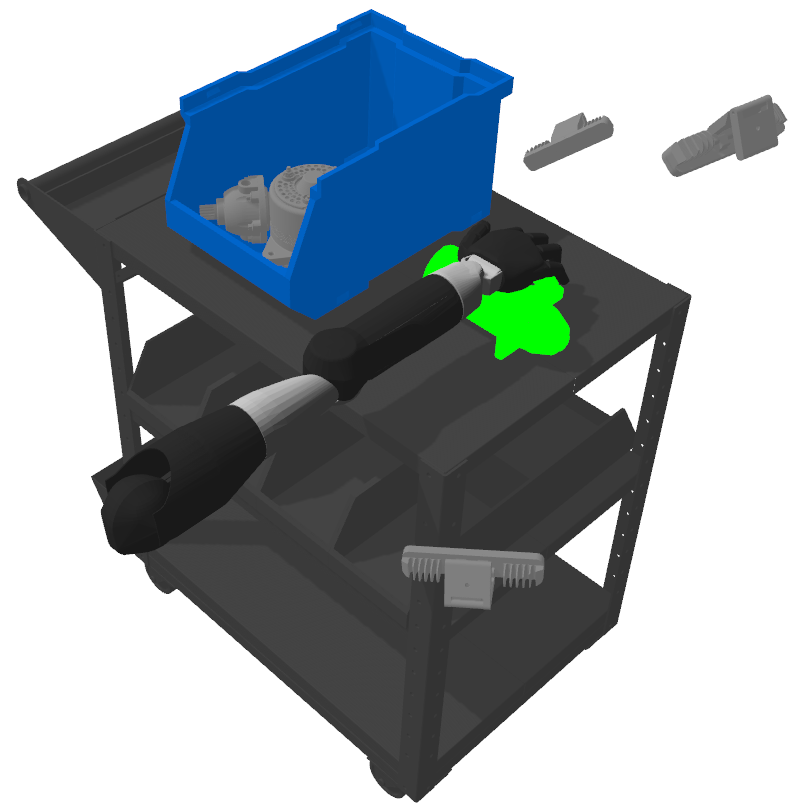
\includegraphics[height=.2\textwidth]{best-views-estimation/active-perception/3-sensors/gazebo-front-right-corner}\hspace{4em}
	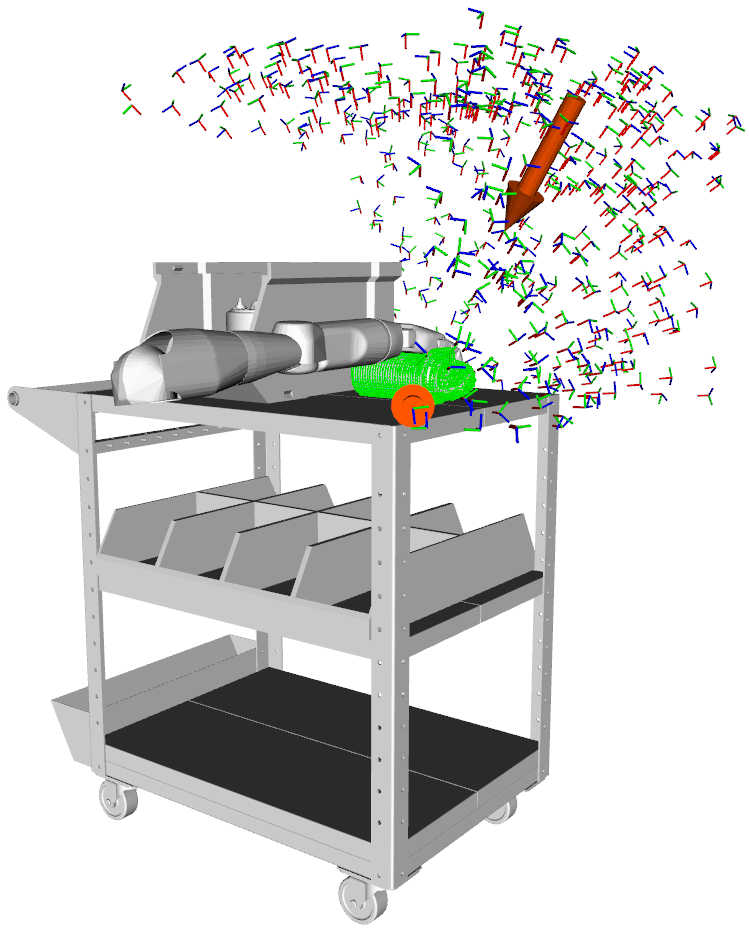
\includegraphics[height=.2\textwidth]{best-views-estimation/active-perception/3-sensors/rviz-front-right}\\
	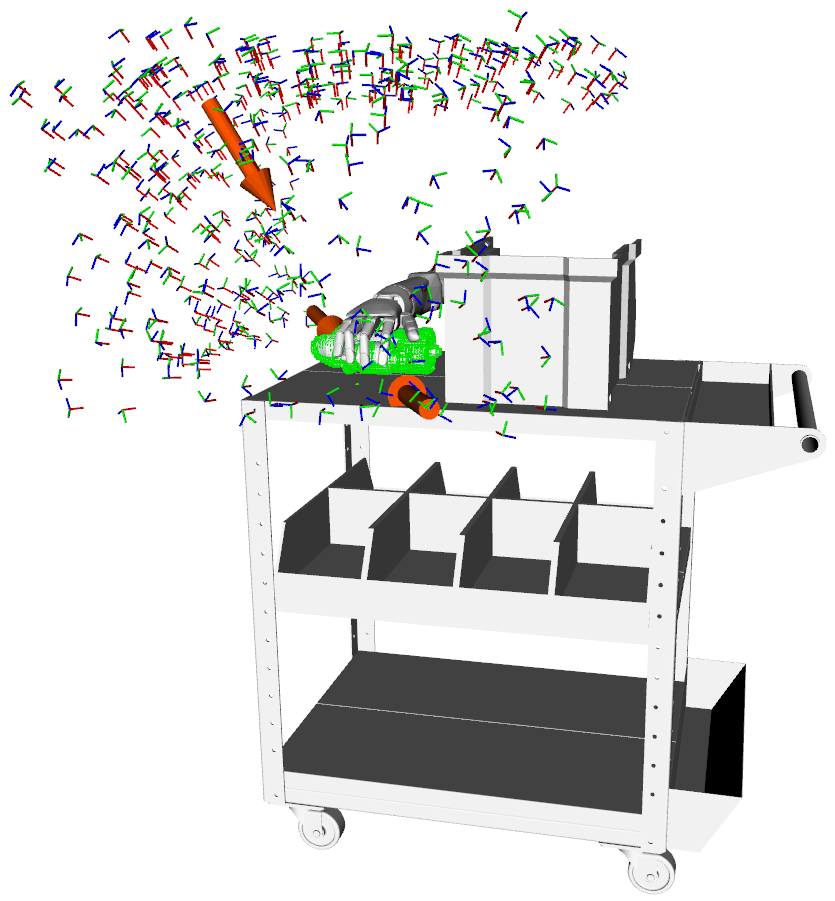
\includegraphics[height=.2\textwidth]{best-views-estimation/active-perception/3-sensors/rviz-back-left}\hspace{2em}
	\includegraphics[height=.2\textwidth]{best-views-estimation/active-perception/3-sensors/rviz-top}
	\caption{Estimation of the 3 best sensors disposition for the active perception environment with a 61.91\% of surface area coverage.}
	\label{fig:active-perception-3-sensors}
\end{figure}

\begin{figure}
	\centering
	\includegraphics[height=.14\textwidth]{best-views-estimation/bin-picking/1-sensor/gazebo-top}\hspace{2em}
	\includegraphics[height=.14\textwidth]{best-views-estimation/bin-picking/1-sensor/rviz-front}\\
	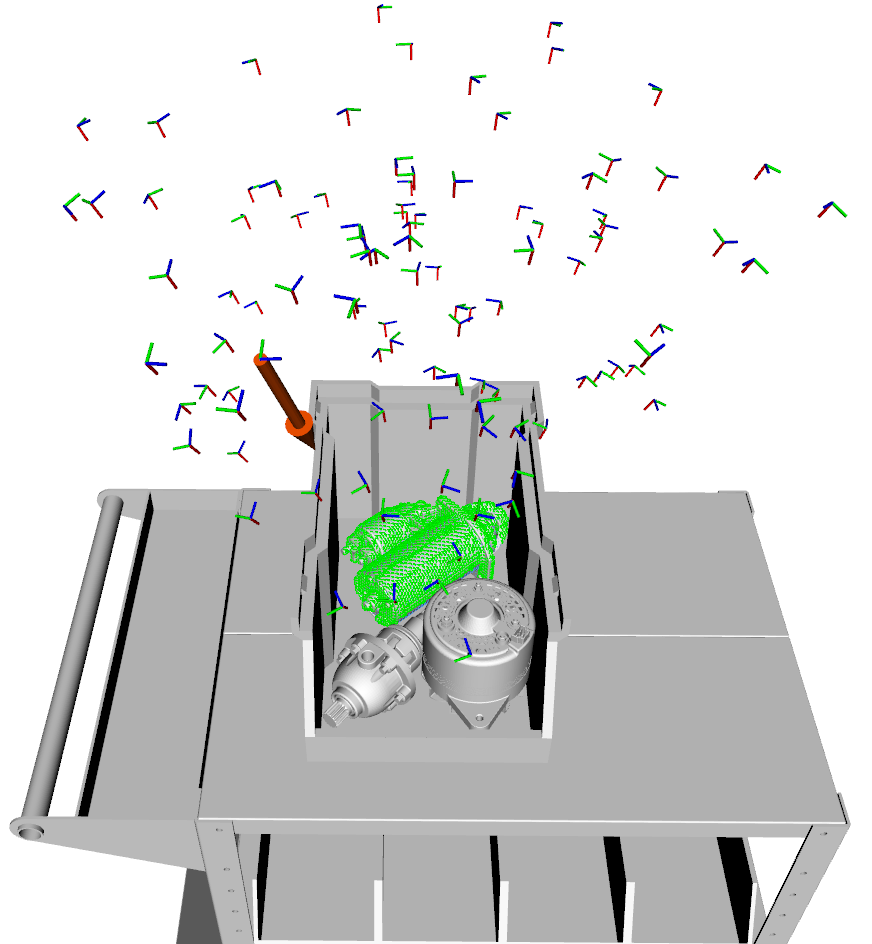
\includegraphics[height=.2\textwidth]{best-views-estimation/bin-picking/1-sensor/rviz-top-front}\hspace{2em}
	\includegraphics[height=.2\textwidth]{best-views-estimation/bin-picking/1-sensor/rviz-top}
	\caption{Estimation of the best sensor position for the bin picking environment with a 45.10\% of surface area coverage.}
	\label{fig:bin-picking-1-sensor}
\end{figure}

\begin{figure}
	\centering
	\includegraphics[height=.19\textwidth]{best-views-estimation/bin-picking/5-sensors/gazebo-front}\hspace{2em}
	\includegraphics[height=.14\textwidth]{best-views-estimation/bin-picking/5-sensors/rviz-top}\\
	\includegraphics[height=.2\textwidth]{best-views-estimation/bin-picking/5-sensors/rviz-corner}\hspace{2em}
	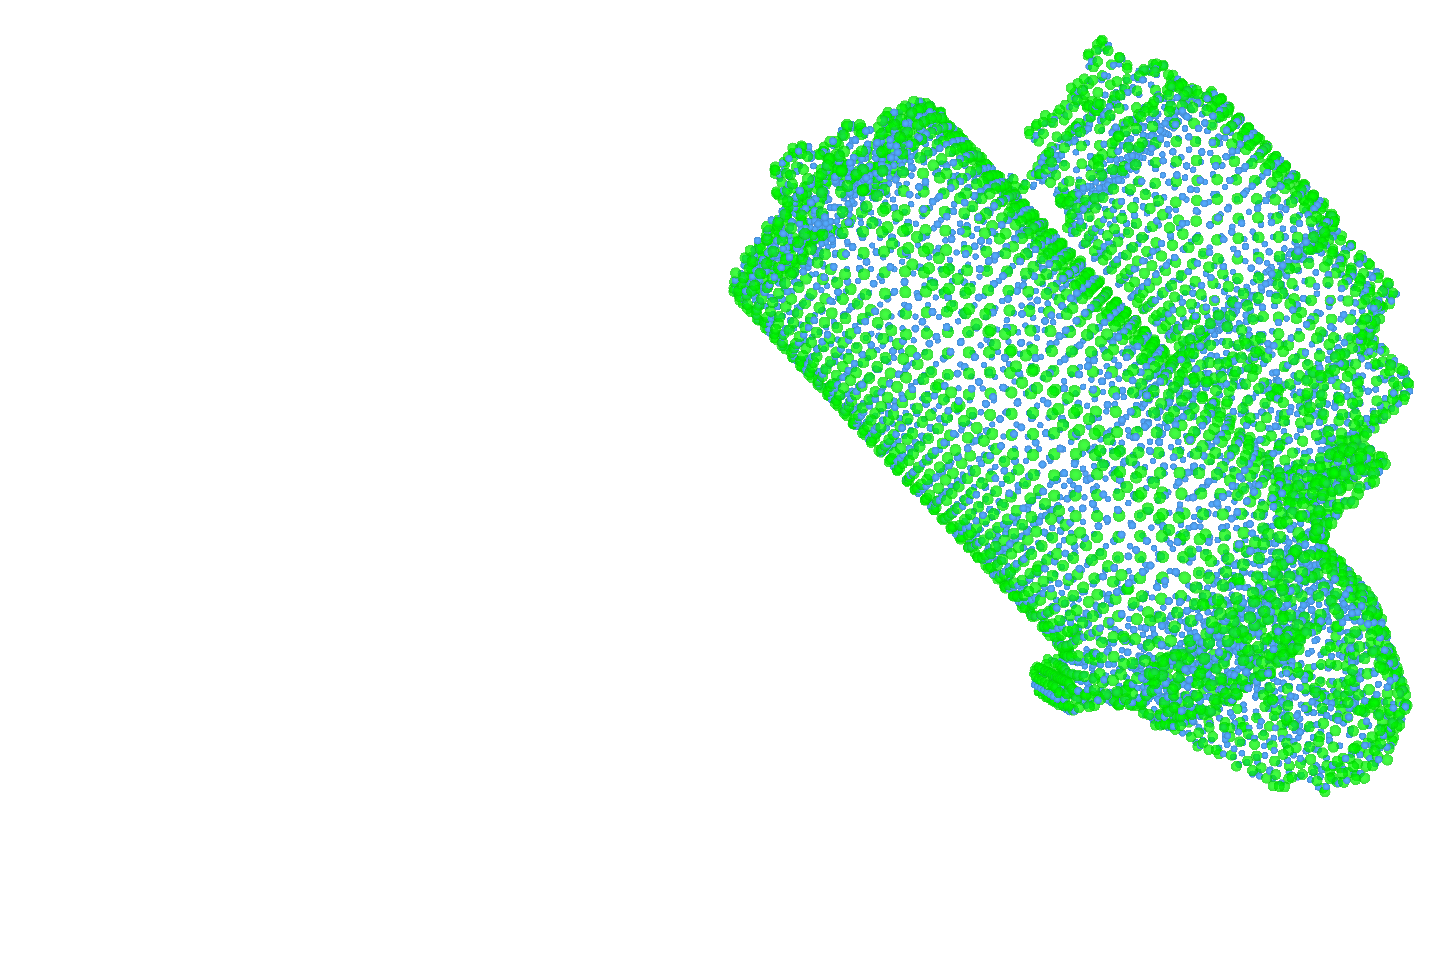
\includegraphics[height=.14\textwidth]{best-views-estimation/bin-picking/5-sensors/rviz-sensor-data}
	\caption{Estimation of the 5 best sensors disposition for the bin picking environment with a 64.63\% of surface area coverage.}
	\label{fig:bin-picking-5-sensors}
\end{figure}

\begin{figure}
	\centering
	\includegraphics[height=.13\textwidth]{best-views-estimation/bin-picking-with-occlusions/1-sensor/gazebo-top}\hspace{2em}
	\includegraphics[height=.13\textwidth]{best-views-estimation/bin-picking-with-occlusions/1-sensor/rviz-corner}\\
	\includegraphics[height=.2\textwidth]{best-views-estimation/bin-picking-with-occlusions/1-sensor/rviz-front}\hspace{2em}
	\includegraphics[height=.2\textwidth]{best-views-estimation/bin-picking-with-occlusions/1-sensor/rviz-top}
	\caption{Estimation of the best sensor position for the bin picking with occlusions environment with a 19.27\% of surface area coverage.}
	\label{fig:bin-picking-with-occlusions-1-sensor}
\end{figure}

\begin{figure}
	\centering
	\includegraphics[height=.18\textwidth]{best-views-estimation/bin-picking-with-occlusions/3-sensors/gazebo-top}\hspace{2em}
	\includegraphics[height=.2\textwidth]{best-views-estimation/bin-picking-with-occlusions/3-sensors/rviz-front}\\
	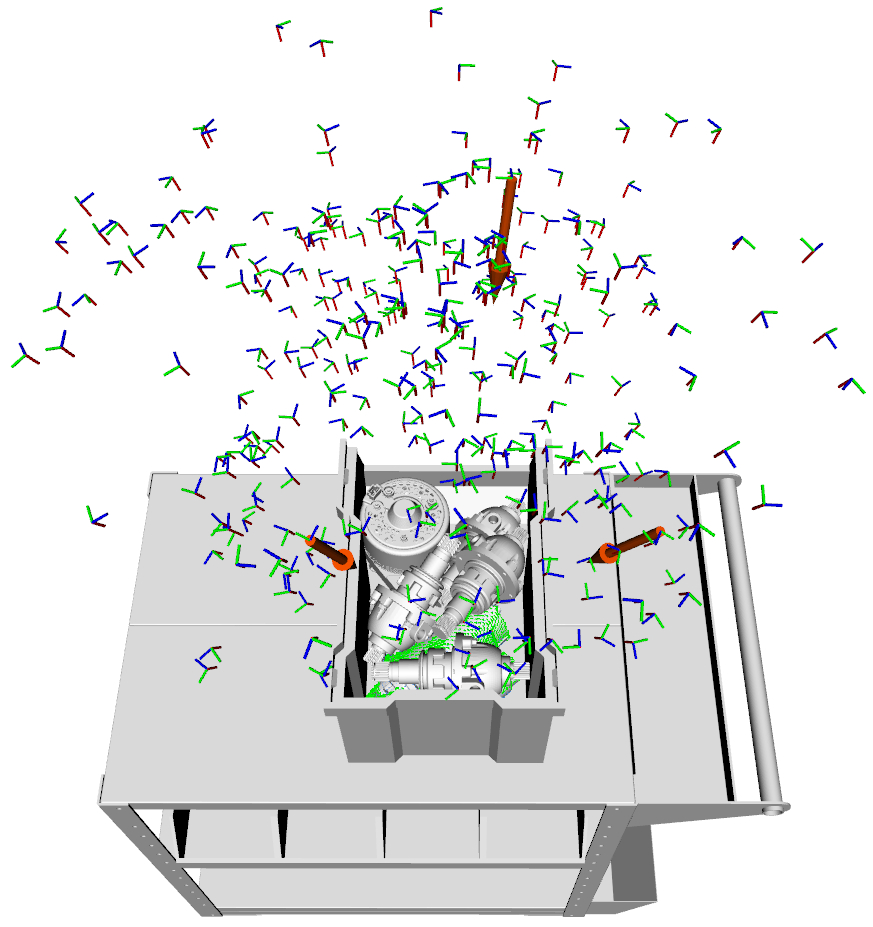
\includegraphics[height=.21\textwidth]{best-views-estimation/bin-picking-with-occlusions/3-sensors/rviz-top-back}\hspace{2em}
	\includegraphics[height=.21\textwidth]{best-views-estimation/bin-picking-with-occlusions/3-sensors/rviz-top}
	\caption{Estimation of the 3 best sensors disposition for the bin picking with occlusions environment with a 31.19\% of surface area coverage.}
	\label{fig:bin-picking-with-occlusions-3-sensors}
\end{figure}

\begin{figure}
	\centering
	\includegraphics[width=.44\textwidth]{best-views-estimation/multiple-bin-picking-with-occlusions/10-sensors/gazebo-front}\vspace{2em}
	\includegraphics[width=.25\textwidth]{best-views-estimation/multiple-bin-picking-with-occlusions/10-sensors/rviz-front-corner}\vspace{2em}
	\includegraphics[width=.43\textwidth]{best-views-estimation/multiple-bin-picking-with-occlusions/10-sensors/rviz-front}\vspace{2em}
	\includegraphics[width=.43\textwidth]{best-views-estimation/multiple-bin-picking-with-occlusions/10-sensors/rviz-top}
	\caption{Estimation of the 10 best sensors disposition for the multiple bin picking with occlusions environment with a 43.93\% of surface area coverage.}
	\label{fig:multiple-bin-picking-with-occlusions-10-sensors}
\end{figure}
